% Options for packages loaded elsewhere
\PassOptionsToPackage{unicode}{hyperref}
\PassOptionsToPackage{hyphens}{url}
%
\documentclass[
]{article}
\usepackage{lmodern}
\usepackage{amssymb,amsmath}
\usepackage{ifxetex,ifluatex}
\ifnum 0\ifxetex 1\fi\ifluatex 1\fi=0 % if pdftex
  \usepackage[T1]{fontenc}
  \usepackage[utf8]{inputenc}
  \usepackage{textcomp} % provide euro and other symbols
\else % if luatex or xetex
  \usepackage{unicode-math}
  \defaultfontfeatures{Scale=MatchLowercase}
  \defaultfontfeatures[\rmfamily]{Ligatures=TeX,Scale=1}
\fi
% Use upquote if available, for straight quotes in verbatim environments
\IfFileExists{upquote.sty}{\usepackage{upquote}}{}
\IfFileExists{microtype.sty}{% use microtype if available
  \usepackage[]{microtype}
  \UseMicrotypeSet[protrusion]{basicmath} % disable protrusion for tt fonts
}{}
\makeatletter
\@ifundefined{KOMAClassName}{% if non-KOMA class
  \IfFileExists{parskip.sty}{%
    \usepackage{parskip}
  }{% else
    \setlength{\parindent}{0pt}
    \setlength{\parskip}{6pt plus 2pt minus 1pt}}
}{% if KOMA class
  \KOMAoptions{parskip=half}}
\makeatother
\usepackage{xcolor}
\IfFileExists{xurl.sty}{\usepackage{xurl}}{} % add URL line breaks if available
\IfFileExists{bookmark.sty}{\usepackage{bookmark}}{\usepackage{hyperref}}
\hypersetup{
  pdftitle={Drawing from the Multivariate Normal Distribution},
  hidelinks,
  pdfcreator={LaTeX via pandoc}}
\urlstyle{same} % disable monospaced font for URLs
\usepackage[margin=1in]{geometry}
\usepackage{color}
\usepackage{fancyvrb}
\newcommand{\VerbBar}{|}
\newcommand{\VERB}{\Verb[commandchars=\\\{\}]}
\DefineVerbatimEnvironment{Highlighting}{Verbatim}{commandchars=\\\{\}}
% Add ',fontsize=\small' for more characters per line
\usepackage{framed}
\definecolor{shadecolor}{RGB}{248,248,248}
\newenvironment{Shaded}{\begin{snugshade}}{\end{snugshade}}
\newcommand{\AlertTok}[1]{\textcolor[rgb]{0.94,0.16,0.16}{#1}}
\newcommand{\AnnotationTok}[1]{\textcolor[rgb]{0.56,0.35,0.01}{\textbf{\textit{#1}}}}
\newcommand{\AttributeTok}[1]{\textcolor[rgb]{0.77,0.63,0.00}{#1}}
\newcommand{\BaseNTok}[1]{\textcolor[rgb]{0.00,0.00,0.81}{#1}}
\newcommand{\BuiltInTok}[1]{#1}
\newcommand{\CharTok}[1]{\textcolor[rgb]{0.31,0.60,0.02}{#1}}
\newcommand{\CommentTok}[1]{\textcolor[rgb]{0.56,0.35,0.01}{\textit{#1}}}
\newcommand{\CommentVarTok}[1]{\textcolor[rgb]{0.56,0.35,0.01}{\textbf{\textit{#1}}}}
\newcommand{\ConstantTok}[1]{\textcolor[rgb]{0.00,0.00,0.00}{#1}}
\newcommand{\ControlFlowTok}[1]{\textcolor[rgb]{0.13,0.29,0.53}{\textbf{#1}}}
\newcommand{\DataTypeTok}[1]{\textcolor[rgb]{0.13,0.29,0.53}{#1}}
\newcommand{\DecValTok}[1]{\textcolor[rgb]{0.00,0.00,0.81}{#1}}
\newcommand{\DocumentationTok}[1]{\textcolor[rgb]{0.56,0.35,0.01}{\textbf{\textit{#1}}}}
\newcommand{\ErrorTok}[1]{\textcolor[rgb]{0.64,0.00,0.00}{\textbf{#1}}}
\newcommand{\ExtensionTok}[1]{#1}
\newcommand{\FloatTok}[1]{\textcolor[rgb]{0.00,0.00,0.81}{#1}}
\newcommand{\FunctionTok}[1]{\textcolor[rgb]{0.00,0.00,0.00}{#1}}
\newcommand{\ImportTok}[1]{#1}
\newcommand{\InformationTok}[1]{\textcolor[rgb]{0.56,0.35,0.01}{\textbf{\textit{#1}}}}
\newcommand{\KeywordTok}[1]{\textcolor[rgb]{0.13,0.29,0.53}{\textbf{#1}}}
\newcommand{\NormalTok}[1]{#1}
\newcommand{\OperatorTok}[1]{\textcolor[rgb]{0.81,0.36,0.00}{\textbf{#1}}}
\newcommand{\OtherTok}[1]{\textcolor[rgb]{0.56,0.35,0.01}{#1}}
\newcommand{\PreprocessorTok}[1]{\textcolor[rgb]{0.56,0.35,0.01}{\textit{#1}}}
\newcommand{\RegionMarkerTok}[1]{#1}
\newcommand{\SpecialCharTok}[1]{\textcolor[rgb]{0.00,0.00,0.00}{#1}}
\newcommand{\SpecialStringTok}[1]{\textcolor[rgb]{0.31,0.60,0.02}{#1}}
\newcommand{\StringTok}[1]{\textcolor[rgb]{0.31,0.60,0.02}{#1}}
\newcommand{\VariableTok}[1]{\textcolor[rgb]{0.00,0.00,0.00}{#1}}
\newcommand{\VerbatimStringTok}[1]{\textcolor[rgb]{0.31,0.60,0.02}{#1}}
\newcommand{\WarningTok}[1]{\textcolor[rgb]{0.56,0.35,0.01}{\textbf{\textit{#1}}}}
\usepackage{graphicx}
\makeatletter
\def\maxwidth{\ifdim\Gin@nat@width>\linewidth\linewidth\else\Gin@nat@width\fi}
\def\maxheight{\ifdim\Gin@nat@height>\textheight\textheight\else\Gin@nat@height\fi}
\makeatother
% Scale images if necessary, so that they will not overflow the page
% margins by default, and it is still possible to overwrite the defaults
% using explicit options in \includegraphics[width, height, ...]{}
\setkeys{Gin}{width=\maxwidth,height=\maxheight,keepaspectratio}
% Set default figure placement to htbp
\makeatletter
\def\fps@figure{htbp}
\makeatother
\setlength{\emergencystretch}{3em} % prevent overfull lines
\providecommand{\tightlist}{%
  \setlength{\itemsep}{0pt}\setlength{\parskip}{0pt}}
\setcounter{secnumdepth}{-\maxdimen} % remove section numbering
\usepackage{mathtools}
\usepackage{amsmath}

\title{Drawing from the Multivariate Normal Distribution}
\usepackage{etoolbox}
\makeatletter
\providecommand{\subtitle}[1]{% add subtitle to \maketitle
  \apptocmd{\@title}{\par {\large #1 \par}}{}{}
}
\makeatother
\subtitle{Derivation, and Programming in R}
\author{}
\date{\vspace{-2.5em}}

\begin{document}
\maketitle

{
\setcounter{tocdepth}{2}
\tableofcontents
}
\hfill\break

\newcommand{\L}{\mathcal{L}}
\newcommand{\bm}[1]{\boldsymbol{#1}}
\newcommand{\argmax}[1]{\mathop{\arg \max}_#1}
\newcommand{\pder}[1]{\dfrac{\partial}{\partial #1}}
\newcommand{\pdertwo}[2]{\dfrac{\partial #1}{\partial #2}}
\newcommand{\d}{\mathrm{d}}
\newcommand{\sumin}{\sum_{i=1}^n}
\newcommand\numberthis{\addtocounter{equation}{1}\tag{\theequation}}
\newcommand{\E}{\mathbb{E}}
\newcommand{\var}{\mathrm{Var}}
\newcommand{\mrm}{\mathrm}
\newcommand{\R}{\mathbb{R}}
\newcommand{\Cov}{\mathrm{Cov}}

\hypertarget{summary}{%
\section{Summary}\label{summary}}

\begin{center}\rule{0.5\linewidth}{0.5pt}\end{center}

To take draws from the multivariate normal distribution, we leverage the
fact that linear transformations of normal random variables are also
normal. By taking a suitable decomposition of the desired covariance
matrix, multiplying this decomposition by independent normal random
vectors, and adding a constant, we can approximate any desired
parameterization of the multivariate normal distriubtion.

\hfill\break

\hypertarget{transformations-of-normal-rvs}{%
\section{Transformations of Normal
RVs}\label{transformations-of-normal-rvs}}

\begin{center}\rule{0.5\linewidth}{0.5pt}\end{center}

\hypertarget{the-univariate-case}{%
\subsubsection{The Univariate Case}\label{the-univariate-case}}

In order to understand how to take draws from a multivariate normal
distribution, it is first important to know that linear transformations
of univariate normal random variables yield normal random variables with
known location and scale parameters. In other words if
\(X \sim \mathcal{N}(\mu, \sigma^2)\) and \(Y = cX + k\), then
\(Y \sim \mathcal{N}(c\mu + k, c^2\sigma^2)\). Proof

\leavevmode\hypertarget{univariate}{}%
~

First, proving that the location and scale parameters are known in the
univariate case is a straightforward application of the fact that
expectations are a linear operator:

\begin{align}
&\text{Let:} \nonumber \\
\nonumber \\
& \quad X \sim \mathcal{N}(\mu,\sigma^2) \nonumber \\[1ex]
& \quad Y = cX + k \quad \text{for constants $c$ and $k$} \nonumber \\
\nonumber \\
&\text{Then:}\nonumber \\
\nonumber \\
&\quad \mathbb{E}(Y) = c\mathbb{E}(X) + k = c\mu + k \nonumber  \\[1ex]
&\quad \mathrm{Var}(Y) = c^2\mathrm{Var}(X) = c^2\sigma^2 \nonumber 
\end{align}

And second, to show that the resulting distribution is univariate
normal, let \(F(\cdot)\) be the (normal) CDF of \(X\) and \(G(\cdot)\)
be the CDF of \(Y\). Then the CDF of Y is:

\begin{align}
G_Y(y) &= \Pr(Y \leq y) \nonumber \\[2ex]
&= \Pr(cX + k \leq y)  \nonumber \\[2ex]
&= \Pr\left(X \leq \frac{y-k}{c}\right) \nonumber \\[2ex]
&= F_X\left(\frac{y-k}{c}\right) \\[2ex]
\end{align}

And differentiating to obtain the pdf of \(Y\): \begin{align}
\implies g_Y(y) &= \dfrac{\partial}{\partial y} F_X\left(\frac{y-k}{c}\right)  \nonumber \\[2ex]
&= f_X\left(\frac{y-k}{c}\right)\frac{1}{c} \nonumber \\[2ex]
\implies f_X\left(\frac{y-k}{c}\right)\frac{1}{c} &= \frac{1}{\sqrt{2\pi}c\sigma} e^{\dfrac{1}{2}\left(\dfrac{\frac{y-k}{c}-\mu}{\sigma}\right)^2} \nonumber \\[2ex]
&=\frac{1}{\sqrt{2\pi}c\sigma} e^{\dfrac{1}{2}\left(\frac{\frac{(cx+k)-k}{c}-\mu}{\sigma}\right)^2}\nonumber \\[2ex]
&=\frac{1}{\sqrt{2\pi}c\sigma} e^{\frac{\left[(cx+k)-(k+c\mu)\right]^2}{2c^2\sigma^2}} \label{pdf.y}
\end{align}

Where \textbackslash ref\{pdf.y\} is clearly a
\(\mathcal{N}(c\mu+k, c^2\sigma^2)\) distribution, which concludes the
proof.

{\(\blacksquare\)}

~

~

Thus, if we multiply \(X\) by the standard deviation that we desire our
transformed variable to have, and then add on a constant, we arrive at
any desired normally distributed random variable. Although this is
somewhat trivial in the univariate case due to software implementations
easily drawing from arbitrary univariate normals, this understanding
proves useful when trying to draw from a multivariate normal
distribution.

\hypertarget{the-multivariate-case}{%
\subsubsection{The Multivariate Case}\label{the-multivariate-case}}

The next step is to extend the univariate case to the multivariate case.
First, let

\begin{align}
\boldsymbol{X} &\sim \mathrm{MVN}(\boldsymbol{\mu}_x, \boldsymbol{\Sigma}_x) \nonumber \\[1ex]
\boldsymbol{Y} &= \boldsymbol{CX} + \boldsymbol{k} \nonumber
\end{align}

Then, it follows that
\[\boldsymbol{Y} \sim \mathrm{MVN}(\boldsymbol{C\mu_x} + \boldsymbol{k}, \boldsymbol{ C\Sigma_x C^\top})\]

where:

\begin{itemize}
\tightlist
\item
  \(\boldsymbol{X}\) is a \(p \times 1\) MVN random vector
\item
  \(\boldsymbol{C}\) is a \(n \times p\) matrix of constants
\item
  \(\boldsymbol{k}\) is a \(n \times 1\) vector of constants
\item
  \(\boldsymbol{\mu}_x\) is the \(p \times 1\) mean vector of
  \(\boldsymbol{X}\)
\item
  \(\boldsymbol{\Sigma}_x\) is the \(p \times p\) covariance matrix of
  \(\boldsymbol{X}\)
\item
  \textbf{Note} that \(p\) can be equal to \(n\)
\end{itemize}

Proof

\leavevmode\hypertarget{MGF}{}%
For proof, recall that the MGF of the MV normal distribution is
\[M_X(t): \mathbb{R}^p \rightarrow \mathbb{R}= \mathbb{E}(e^{t^\top X}) = e^{t^\top \boldsymbol{\mu }+ \frac{1}{2}t^\top \boldsymbol{\Sigma }t}\]
for \(t \in \mathbb{R}^p\).

Then for \(t \in \mathbb{R}^n\) (dropping bold for matrices and
vectors), the joint MGF of \(Y\),
\(M_Y(t): \mathbb{R}^n \rightarrow \mathbb{R}\), is:

\begin{align}
M_Y(t) &= \mathbb{E}(e^{t^\top Y}) \\[2ex]
       &= \mathbb{E}\left(e^{t^\top(CX + k)}\right) \nonumber \\[2ex]
&=  \mathbb{E}\left(e^{t^\top CX}e^{t^\top k}\right) \nonumber \\[2ex]
&= e^{t^\top k}\mathbb{E}\left(e^{t^\top CX}\right) \nonumber \\[2ex]
&= e^{t^\top k} M_X(tC) \nonumber \\[2ex]
&= e^{t^\top k} e^{t^\top C \mu + \frac{1}{2}t^\top C \Sigma C^\top t} \nonumber \\[2ex]
&= e^{ t^\top k + t^\top C \mu  + \frac{1}{2}t^\top C \Sigma C^\top t} \nonumber \\[2ex]
&= e^{t^\top (C \mu + k) + \frac{1}{2}t^\top C \Sigma C^\top t} \label{mgf}
\end{align}

And, equation \textbackslash ref\{mgf\} is clearly the MGF of a
\(\mathrm{MVN}(\boldsymbol{C\mu + k}, \boldsymbol{C\Sigma C^\top})\)
distribution, which by the MGF Uniqueness Theorem implies that \(Y\) has
this distribution, which concludes the proof.

{\(\blacksquare\)}

\hfill\break

\hypertarget{generating-from-the-mv-normal}{%
\section{Generating from the MV
Normal}\label{generating-from-the-mv-normal}}

\begin{center}\rule{0.5\linewidth}{0.5pt}\end{center}

\textbf{Note}: The exposition here relies on a bivariate normal,
although this readily extends to arbitrarily large dimensions.

From the above result regarding transformations of MVN random variables,
it is clear that if we first generate independent univariate normals,
and then choose a matrix \(\boldsymbol{C}\) and vector
\(\boldsymbol{k}\) carefully, we can generate any arbitrary multivariate
normal sample. First, to obtain the desired mean, we can simply add a
vector of constants to \(\boldsymbol{X}\), eg
\(\boldsymbol{X} + \boldsymbol{k}\). However, to get the desired
covariance structure is a bit more involved. From the above proof we
have that

\begin{align}
\boldsymbol{X} &\sim \mathrm{MVN}(\boldsymbol{\mu}_x, \boldsymbol{\Sigma}_x) \nonumber \\[1ex]
\boldsymbol{Y} &= \boldsymbol{CX} + \boldsymbol{k} \nonumber \\[1.5ex]
\implies \boldsymbol{Y} &\sim \mathrm{MVN}(\boldsymbol{C\mu_x} + \boldsymbol{k}, \boldsymbol{ C\Sigma_x C^\top})
\end{align}

Now, suppose we generate the observations on \(\boldsymbol{X}\) as
i.i.d. standard normal random variables: \begin{align}
\boldsymbol{\mu }&= (0,0) \nonumber \\[1.5ex]
\boldsymbol{\Sigma }&= \begin{bmatrix}
1 & 0 \\
0 & 1 
\end{bmatrix} \nonumber 
\end{align}

Then we have that \(\boldsymbol{\Sigma}_x = \boldsymbol{I}\), so to
obtain multivariate normal samples with any desired covariance
structure, we simply have to find a suitable matrix \(\boldsymbol{C}\)
by which we can multiply the i.i.d. standard normal variables in
\(\boldsymbol{X}\). Doing so will yield the random vector
\(\boldsymbol{Y}\) with covariance
\[\mathrm{Cov}(\boldsymbol{Y}) = \boldsymbol{C\Sigma_x C}^\top = \boldsymbol{CIC}^\top = \boldsymbol{CC}^\top\]
as already proven. Importantly, note that the matrix square- root of a
matrix \(\boldsymbol{A}\) is any matrix \(\boldsymbol{B}\) such that
\(BB^\top = A\).\footnote{This is an alternative definition of the
  matrix square-root. More often, it is defined as \(A=BB\) instead of
  \(A=BB^\top\)} This implies that the matrix of constants,
\(\boldsymbol{C}\), by which we multiply \(\boldsymbol{X}\) is in fact
the matrix square-root of \(\boldsymbol{\Sigma}_y\), directly analogous
to the univariate case in which we multiplied \(X\) by the standard
deviation of our desired covariance.

Thus, the steps to generate from any multivariate normal distribution
are:

\begin{enumerate}
\def\labelenumi{\arabic{enumi}.}
\item
  Decide on a desired covariance matrix, \(\boldsymbol{\Sigma}_y\)
\item
  Decide on a desired mean vector,
  \(\boldsymbol{\mu}_y = \boldsymbol{k}\)
\item
  Generate \(\boldsymbol{X}\) as independent standard normal \((0,1)\)
  random variables
\item
  Obtain the matrix square-root, \(\boldsymbol{C}\), of
  \(\boldsymbol{\Sigma}_y\) (so that
  \(\boldsymbol{CC}^\top = \boldsymbol{\Sigma}_y\))
\item
  Multiply \(\boldsymbol{CX}\) and add
  \(\boldsymbol{CX} + \boldsymbol{k}\)
\end{enumerate}

To find the matrix square-root of \(\boldsymbol{\Sigma}_y\) which will
serve as the matrix of constants, \(\boldsymbol{C}\), by which we
multiply \(\boldsymbol{X}\), two factorizations of
\(\boldsymbol{\Sigma}_y = \boldsymbol{CC^\top}\) immediately come to
mind, although several others can also work:

\begin{enumerate}
\def\labelenumi{\arabic{enumi}.}
\item
  \textbf{Cholesky decomposition} -- \(LL^\top\) where \(L\) is
  lower-triangular. This is unique for positive definite matrices, which
  all valid covariance matrices are.
\item
  \textbf{Singular values decomposition} (SVD) -- \(UDV^\top\), where
  \(U\) and \(V\) are orthogonal matrices whose columns are the left and
  right singular vectors, and \(D\) is a diagonal matrix containing the
  singular values. Because of the orthogonal and diagonal matrices, this
  is geometrically a rotation, dilation, and rotation. \textbf{Note}
  that for real, symmetric, positive-definite matrices, this is
  identical to the spectral decomposition.
\end{enumerate}

\hfill\break

\hypertarget{via-cholesky}{%
\subsubsection{Via Cholesky}\label{via-cholesky}}

\begin{center}\rule{0.5\linewidth}{0.5pt}\end{center}

To obtain the matrix square-root, \(\boldsymbol{C}\), via the Cholesky
decomposition decompose \(\boldsymbol{\Sigma}_y\) as
\[\boldsymbol{\Sigma}_y = \boldsymbol{LL}^\top\] and multiply
\[\boldsymbol{LX}\] which yields
\[\boldsymbol{Y} \sim (\boldsymbol{0}, \boldsymbol{LL^\top})\] which has
exactly the covariance structure that we wanted, as \(\boldsymbol{L}\)
is equivalent to the matrix \(\boldsymbol{C}\) that we were looking for.

\hfill\break

\hypertarget{via-svd}{%
\subsubsection{Via SVD}\label{via-svd}}

\begin{center}\rule{0.5\linewidth}{0.5pt}\end{center}

For the SVD, decompose \(\boldsymbol{\Sigma}_y\) as
\[\boldsymbol{\Sigma}_y = \boldsymbol{UDV}^\top = \boldsymbol{UDU}^\top\]
The last equality follows in this case because \(\Sigma_y\) is a
symmetric, positive definite matrix. Proof

\leavevmode\hypertarget{SVD}{}%
\hfill\break

Suppose we take the SVD of a symmetric matrix \(A\). Then the left
singluar vectors, \(U\), are the eigenvectors of \(AA^\top\), while the
right singular vectors, \(V\), are the eigenvectors of \(A^\top A\) (see
\href{https://math.mit.edu/classes/18.095/2016IAP/lec2/SVD_Notes.pdf}{this}
link for proof). However, since \(A\) is symmetric,
\[A = A^\top \implies AA^\top = A^\top A \implies U = V\]

{\(\blacksquare\)}

\hfill\break

Finally, pre-multiplying the univariate normals in \(X\) by the matrix
square-root, \(C\), of \(\Sigma_y\) yields (dropping bolding)

\begin{align}
Y= CX &= UD^{1/2} X \nonumber \\[1ex]
\implies Y &\sim \left(\boldsymbol{0}, UD^{1/2}\boldsymbol{\Sigma }(UD^{1/2})^\top \right) \nonumber \\[1ex]
& \sim \left(\boldsymbol{0}, UD^{1/2}\boldsymbol{I} (UD^{1/2})^\top \right) \nonumber \\[1ex]
& \sim \left(\boldsymbol{0}, UD^{1/2}D^{1/2}U^\top\right) \nonumber \\[1ex]
& \sim \left(\boldsymbol{0} , UDU^\top\right) \nonumber \\[1ex]
& \sim \left(\boldsymbol{0} , \boldsymbol{\Sigma}_y\right) \nonumber \\[1ex]
\end{align}

So to obtain the desired covariance \(\boldsymbol{\Sigma}_y\) from \(X\)
we simply set \(\boldsymbol{C} = \boldsymbol{UD}^{1/2}\) and premultiply
\(\boldsymbol{CX}\).\footnote{We could also use
  \(\boldsymbol{UD^{1/2}U^\top}\) as the matrix square-root, although
  this requires more computations.}

\hfill\break

\hypertarget{programming-in-r}{%
\section{Programming in R}\label{programming-in-r}}

\begin{center}\rule{0.5\linewidth}{0.5pt}\end{center}

To do this in R, we follow the steps outlined previously. Thus, we first
decide on the desired mean vector, \(\boldsymbol{\mu}_y\), and
covariance matrix, \(\boldsymbol{\Sigma}_y\). Recall also that a valid,
full-rank covariance matrix is positive-definite.\footnote{An
  interesting way to understand why (other than mathematical necessity)
  is that the correlation between some of the variables would be
  \(\geq 1\) or \(\leq -1\) if this did not hold, which is not a valid
  correlation.}

\begin{Shaded}
\begin{Highlighting}[]
\NormalTok{mu.y =}\StringTok{ }\KeywordTok{c}\NormalTok{(}\OperatorTok{{-}}\NormalTok{.}\DecValTok{246}\NormalTok{, }\FloatTok{{-}1.3}\NormalTok{, }\FloatTok{1.645}\NormalTok{)}

\NormalTok{sigma.y =}\StringTok{ }\KeywordTok{matrix}\NormalTok{(}\KeywordTok{c}\NormalTok{(}\DecValTok{2}\NormalTok{,    }\FloatTok{.66}\NormalTok{, }\FloatTok{{-}1.2}\NormalTok{,}
                   \FloatTok{.66}\NormalTok{,  }\FloatTok{.75}\NormalTok{, }\FloatTok{{-}.75}\NormalTok{,}
                  \FloatTok{{-}1.2}\NormalTok{, }\FloatTok{{-}.75}\NormalTok{,  }\FloatTok{2.5}\NormalTok{),}
                 \DataTypeTok{nrow =} \DecValTok{3}\NormalTok{, }\DataTypeTok{byrow=}\NormalTok{T)}
\CommentTok{\#desired cov}
\NormalTok{sigma.y}
\end{Highlighting}
\end{Shaded}

\begin{verbatim}
##       [,1]  [,2]  [,3]
## [1,]  2.00  0.66 -1.20
## [2,]  0.66  0.75 -0.75
## [3,] -1.20 -0.75  2.50
\end{verbatim}

\begin{Shaded}
\begin{Highlighting}[]
\CommentTok{\#check pos def}
\KeywordTok{all}\NormalTok{(}\KeywordTok{eigen}\NormalTok{(sigma.y)}\OperatorTok{$}\NormalTok{values }\OperatorTok{\textgreater{}}\StringTok{ }\DecValTok{0}\NormalTok{)}
\end{Highlighting}
\end{Shaded}

\begin{verbatim}
## [1] TRUE
\end{verbatim}

~

Second, we'll simulate some i.i.d. multivariate standard normal data in
3 dimensions.

\begin{Shaded}
\begin{Highlighting}[]
\CommentTok{\#simulate trivariate iid standard normal }
\NormalTok{n =}\StringTok{ }\DecValTok{10000}
\NormalTok{x =}\StringTok{ }\KeywordTok{matrix}\NormalTok{(}\KeywordTok{rnorm}\NormalTok{(n}\OperatorTok{*}\DecValTok{3}\NormalTok{), }\DataTypeTok{nrow=}\DecValTok{3}\NormalTok{)}
\end{Highlighting}
\end{Shaded}

\hfill\break

And then finally we take the Cholesky and SVD of the desired covariance,
multiply \(\boldsymbol{X}\) by the appropriate matrix
\(\boldsymbol{C}\), and then add on the constant to get the desired
mean.

\begin{Shaded}
\begin{Highlighting}[]
\CommentTok{\#Via cholesky}
\NormalTok{chol.sig.y =}\StringTok{ }\KeywordTok{chol.default}\NormalTok{(sigma.y)}
\NormalTok{y.chol =}\StringTok{ }\KeywordTok{t}\NormalTok{(chol.sig.y) }\OperatorTok{\%*\%}\StringTok{ }\NormalTok{x }\CommentTok{\# R returns the upper{-}triangular, L\^{}t by default}

\CommentTok{\#Via svd}
\NormalTok{svd.sig.y =}\StringTok{ }\KeywordTok{svd}\NormalTok{(sigma.y)}
\NormalTok{u =}\StringTok{ }\NormalTok{svd.sig.y}\OperatorTok{$}\NormalTok{u}
\NormalTok{d =}\StringTok{ }\NormalTok{svd.sig.y}\OperatorTok{$}\NormalTok{d}
\NormalTok{svd.sig.y =}\StringTok{ }\NormalTok{u}\OperatorTok{\%*\%}\KeywordTok{diag}\NormalTok{(d)}\OperatorTok{\^{}}\NormalTok{(}\DecValTok{1}\OperatorTok{/}\DecValTok{2}\NormalTok{)}
\NormalTok{y.svd =}\StringTok{  }\NormalTok{svd.sig.y }\OperatorTok{\%*\%}\StringTok{ }\NormalTok{x }

\CommentTok{\# add on mean }
\CommentTok{\#(transpose for taking the covariance of a matrix in R on next lines)}
\NormalTok{y.svd =}\StringTok{ }\KeywordTok{t}\NormalTok{(y.svd }\OperatorTok{+}\StringTok{ }\NormalTok{mu.y)}
\NormalTok{y.chol =}\StringTok{ }\KeywordTok{t}\NormalTok{(y.chol }\OperatorTok{+}\StringTok{ }\NormalTok{mu.y)}

\CommentTok{\# results }
\KeywordTok{list}\NormalTok{(}\DataTypeTok{chol =} \KeywordTok{list}\NormalTok{(}\DataTypeTok{mean=}\KeywordTok{apply}\NormalTok{(y.chol, }\DecValTok{2}\NormalTok{, mean),}
                 \DataTypeTok{cov=}\KeywordTok{cov}\NormalTok{(y.chol)),}
     \DataTypeTok{svd  =} \KeywordTok{list}\NormalTok{(}\DataTypeTok{mean=}\KeywordTok{apply}\NormalTok{(y.svd, }\DecValTok{2}\NormalTok{, mean),}
                 \DataTypeTok{cov=}\KeywordTok{cov}\NormalTok{(y.svd)),}
     \DataTypeTok{desired =}\NormalTok{ sigma.y)}
\end{Highlighting}
\end{Shaded}

\begin{verbatim}
## $chol
## $chol$mean
## [1] -0.2298272 -1.2878447  1.6175183
## 
## $chol$cov
##            [,1]       [,2]       [,3]
## [1,]  1.9732459  0.6422516 -1.1752526
## [2,]  0.6422516  0.7358982 -0.7333378
## [3,] -1.1752526 -0.7333378  2.4505213
## 
## 
## $svd
## $svd$mean
## [1] -0.2505706 -1.3129560  1.6661188
## 
## $svd$cov
##           [,1]       [,2]       [,3]
## [1,]  1.991494  0.6551940 -1.1855894
## [2,]  0.655194  0.7376814 -0.7363857
## [3,] -1.185589 -0.7363857  2.4522149
## 
## 
## $desired
##       [,1]  [,2]  [,3]
## [1,]  2.00  0.66 -1.20
## [2,]  0.66  0.75 -0.75
## [3,] -1.20 -0.75  2.50
\end{verbatim}

\hfill\break

From the above output, it is clear that the desired covariance structure
is approximated fairly well.

\hfill\break

\hypertarget{which-is-better}{%
\subsubsection{Which is better}\label{which-is-better}}

We've learned that two factorizations work, but which one is ``better,''
numerically? This may depend on how we define ``better,'' but lets try
and find out. First, for simplicity we will only look at the accuracy of
the covariance. Second, lets say that a factorization is better if it
minimizes \(max_{ij} |Cov(x_{i}, x_{j}) - D_{ij}|\) where \(D_{ij}\) is
each element of the desired covariance matrix. That is, which method
minimizes the maximum absolute deviation from the desired covariance
structure.

Taking this objective in mind, we can explore this by the monte carlo
method. We'll first define a function that returns the value of the
objective, as well as the sample size, and decomposition used, and then
compare the loss after several iterations for each sample size.

\begin{Shaded}
\begin{Highlighting}[]
\NormalTok{mv.loss =}\StringTok{ }\ControlFlowTok{function}\NormalTok{(n, sigma.y)\{}
\NormalTok{  n =}\StringTok{ }\NormalTok{n}
\NormalTok{  x =}\StringTok{ }\KeywordTok{matrix}\NormalTok{(}\KeywordTok{rnorm}\NormalTok{(n}\OperatorTok{*}\DecValTok{3}\NormalTok{), }\DataTypeTok{nrow=}\DecValTok{3}\NormalTok{)}


  \CommentTok{\# chol}
\NormalTok{  chol.sig.y =}\StringTok{ }\KeywordTok{chol.default}\NormalTok{(sigma.y)}
\NormalTok{  y.chol =}\StringTok{ }\KeywordTok{t}\NormalTok{(chol.sig.y) }\OperatorTok{\%*\%}\StringTok{ }\NormalTok{x }

\NormalTok{  loss.chol =}\StringTok{ }\KeywordTok{max}\NormalTok{( }\KeywordTok{abs}\NormalTok{( }\KeywordTok{cov}\NormalTok{(}\KeywordTok{t}\NormalTok{(y.chol)) }\OperatorTok{{-}}\StringTok{ }\NormalTok{sigma.y) )}

  \CommentTok{\# Via svd}
\NormalTok{  svd.sig.y =}\StringTok{ }\KeywordTok{svd}\NormalTok{(sigma.y)}
\NormalTok{  u =}\StringTok{ }\NormalTok{svd.sig.y}\OperatorTok{$}\NormalTok{u}
\NormalTok{  d =}\StringTok{ }\NormalTok{svd.sig.y}\OperatorTok{$}\NormalTok{d}
\NormalTok{  svd.sig.y =}\StringTok{ }\NormalTok{u}\OperatorTok{\%*\%}\KeywordTok{diag}\NormalTok{(d)}\OperatorTok{\^{}}\NormalTok{(}\DecValTok{1}\OperatorTok{/}\DecValTok{2}\NormalTok{)}
\NormalTok{  y.svd =}\StringTok{  }\NormalTok{svd.sig.y }\OperatorTok{\%*\%}\StringTok{ }\NormalTok{x }

\NormalTok{  loss.svd =}\StringTok{ }\KeywordTok{max}\NormalTok{( }\KeywordTok{abs}\NormalTok{( }\KeywordTok{cov}\NormalTok{(}\KeywordTok{t}\NormalTok{(y.svd)) }\OperatorTok{{-}}\StringTok{ }\NormalTok{sigma.y) )}

\KeywordTok{return}\NormalTok{(}\KeywordTok{c}\NormalTok{(}\DataTypeTok{chol =}\NormalTok{ loss.chol, }\DataTypeTok{svd =}\NormalTok{ loss.svd, }\DataTypeTok{n=}\NormalTok{n))}

\NormalTok{\}}
\end{Highlighting}
\end{Shaded}

\hfill\break

And lets make sure its working as expected, using the desired covariance
previously defined:

\begin{Shaded}
\begin{Highlighting}[]
\KeywordTok{mv.loss}\NormalTok{(}\DataTypeTok{n =} \DecValTok{100}\NormalTok{, }\DataTypeTok{sigma.y =}\NormalTok{ sigma.y)}
\end{Highlighting}
\end{Shaded}

\begin{verbatim}
##        chol         svd           n 
##   0.3783253   0.7861566 100.0000000
\end{verbatim}

\hfill\break

And finally, now that we know the function works, we can do several
iterations at each sample size to see which method converges fastest.

\begin{Shaded}
\begin{Highlighting}[]
\CommentTok{\# get things ready for parallel run, plotting}
\NormalTok{pks =}\StringTok{ }\KeywordTok{c}\NormalTok{(}\StringTok{"parallel"}\NormalTok{, }\StringTok{"dplyr"}\NormalTok{, }\StringTok{"ggplot2"}\NormalTok{, }\StringTok{"reshape2"}\NormalTok{)}
\KeywordTok{invisible}\NormalTok{(}\KeywordTok{sapply}\NormalTok{(pks, library, }\DataTypeTok{character.only=}\NormalTok{T))}

\KeywordTok{RNGkind}\NormalTok{(}\StringTok{"L\textquotesingle{}Ecuyer{-}CMRG"}\NormalTok{) }\CommentTok{\# for parallel reproducibility}
\KeywordTok{set.seed}\NormalTok{(}\DecValTok{167492}\NormalTok{)}

\CommentTok{\#Grid of sample sizes}
\NormalTok{niter =}\StringTok{ }\DecValTok{10000}
\NormalTok{n =}\StringTok{ }\KeywordTok{c}\NormalTok{(}\DecValTok{30}\NormalTok{, }\DecValTok{60}\NormalTok{, }\DecValTok{125}\NormalTok{, }\DecValTok{250}\NormalTok{, }\DecValTok{500}\NormalTok{, }\DecValTok{750}\NormalTok{, }\DecValTok{1000}\NormalTok{, }\DecValTok{2500}\NormalTok{, }\DecValTok{5000}\NormalTok{, }\DecValTok{7500}\NormalTok{, }\DecValTok{10000}\NormalTok{)}
\NormalTok{n.grid =}\StringTok{ }\KeywordTok{rep}\NormalTok{(n, }\DataTypeTok{each =}\NormalTok{ niter)}

\CommentTok{\# run sims, summarize, plot}
\NormalTok{res =}\StringTok{ }\KeywordTok{mclapply}\NormalTok{(n.grid, mv.loss, }\DataTypeTok{sigma.y=}\NormalTok{sigma.y, }
               \DataTypeTok{mc.preschedule=}\NormalTok{T,}
               \DataTypeTok{mc.cores =}\NormalTok{ (parallel}\OperatorTok{::}\KeywordTok{detectCores}\NormalTok{()}\OperatorTok{{-}}\DecValTok{1}\NormalTok{))}

\NormalTok{dat =}\StringTok{ }\KeywordTok{as.data.frame}\NormalTok{(}\KeywordTok{do.call}\NormalTok{(rbind, res))}

\NormalTok{summaries =}\StringTok{ }\NormalTok{dat }\OperatorTok{\%\textgreater{}\%}\StringTok{ }
\StringTok{  }\KeywordTok{group\_by}\NormalTok{(n) }\OperatorTok{\%\textgreater{}\%}\StringTok{ }
\StringTok{  }\KeywordTok{summarise}\NormalTok{(}\DataTypeTok{mean.chol =} \KeywordTok{mean}\NormalTok{(chol),}
            \DataTypeTok{mean.svd  =} \KeywordTok{mean}\NormalTok{(svd))}

\NormalTok{summaries =}\StringTok{ }\KeywordTok{melt}\NormalTok{(summaries, }
                 \DataTypeTok{id.vars=}\StringTok{"n"}\NormalTok{, }
                 \DataTypeTok{measure.vars =} \KeywordTok{c}\NormalTok{(}\StringTok{"mean.chol"}\NormalTok{,}
                                  \StringTok{"mean.svd"}\NormalTok{))}

\NormalTok{summaries}\OperatorTok{$}\NormalTok{n =}\StringTok{ }\KeywordTok{as.factor}\NormalTok{(summaries}\OperatorTok{$}\NormalTok{n)}

\KeywordTok{ggplot}\NormalTok{(}\DataTypeTok{data=}\NormalTok{summaries, }\KeywordTok{aes}\NormalTok{(}\DataTypeTok{x=}\NormalTok{n)) }\OperatorTok{+}
\StringTok{  }\KeywordTok{geom\_point}\NormalTok{(}\KeywordTok{aes}\NormalTok{(}\DataTypeTok{y =}\NormalTok{ value, }\DataTypeTok{color=}\NormalTok{variable, }\DataTypeTok{shape=}\NormalTok{variable),}
             \DataTypeTok{position=}\KeywordTok{position\_dodge}\NormalTok{(}\DataTypeTok{width=}\NormalTok{.}\DecValTok{5}\NormalTok{),}
             \DataTypeTok{size=}\DecValTok{3}\NormalTok{) }\OperatorTok{+}
\StringTok{  }\KeywordTok{theme\_bw}\NormalTok{() }\OperatorTok{+}
\StringTok{  }\KeywordTok{scale\_color\_brewer}\NormalTok{(}\DataTypeTok{palette =} \StringTok{"Set1"}\NormalTok{, }\DataTypeTok{labels =} \KeywordTok{c}\NormalTok{(}\StringTok{"Cholesky"}\NormalTok{, }\StringTok{"SVD"}\NormalTok{)) }\OperatorTok{+}
\StringTok{  }\KeywordTok{scale\_shape\_discrete}\NormalTok{(}\DataTypeTok{labels=}\KeywordTok{c}\NormalTok{(}\StringTok{"Cholesky"}\NormalTok{, }\StringTok{"SVD"}\NormalTok{)) }\OperatorTok{+}
\StringTok{  }\KeywordTok{labs}\NormalTok{(}\DataTypeTok{title=}\StringTok{"Average of Max Absolute Deviation for Covariance of MVN"}\NormalTok{,}
       \DataTypeTok{subtitle =} \StringTok{"Cholesky vs. SVD"}\NormalTok{,}
       \DataTypeTok{x=} \StringTok{"N"}\NormalTok{,}
       \DataTypeTok{y=} \StringTok{"Max Absolute Deviation"}\NormalTok{,}
       \DataTypeTok{color =} \StringTok{"Method"}\NormalTok{,}
       \DataTypeTok{shape =} \StringTok{"Method"}\NormalTok{) }\OperatorTok{+}
\StringTok{  }\KeywordTok{theme}\NormalTok{(}\DataTypeTok{panel.grid.major =} \KeywordTok{element\_blank}\NormalTok{(),}
        \DataTypeTok{legend.position =} \KeywordTok{c}\NormalTok{(.}\DecValTok{85}\NormalTok{,.}\DecValTok{85}\NormalTok{)) }
\end{Highlighting}
\end{Shaded}

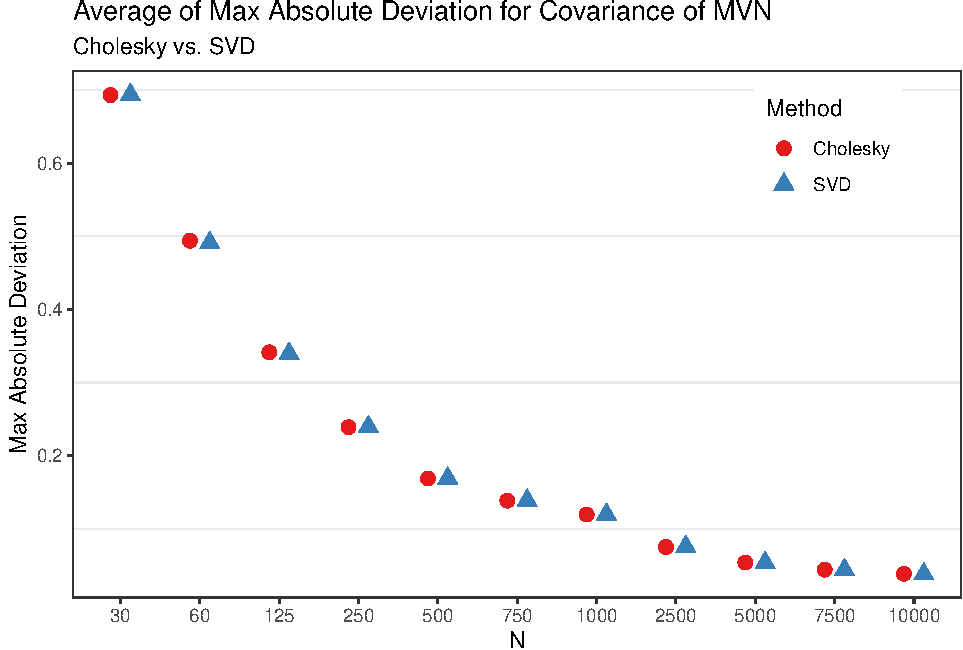
\includegraphics{mvnorm_files/figure-latex/unnamed-chunk-6-1.pdf}

\hfill\break

From these results, it appears as though the two perform roughly the
same in terms of max absolute deviations from the desired covariance
structure, on average. However, it looks like they may be slightly
different in small samples, so lets take a look to be sure.

\hfill\break

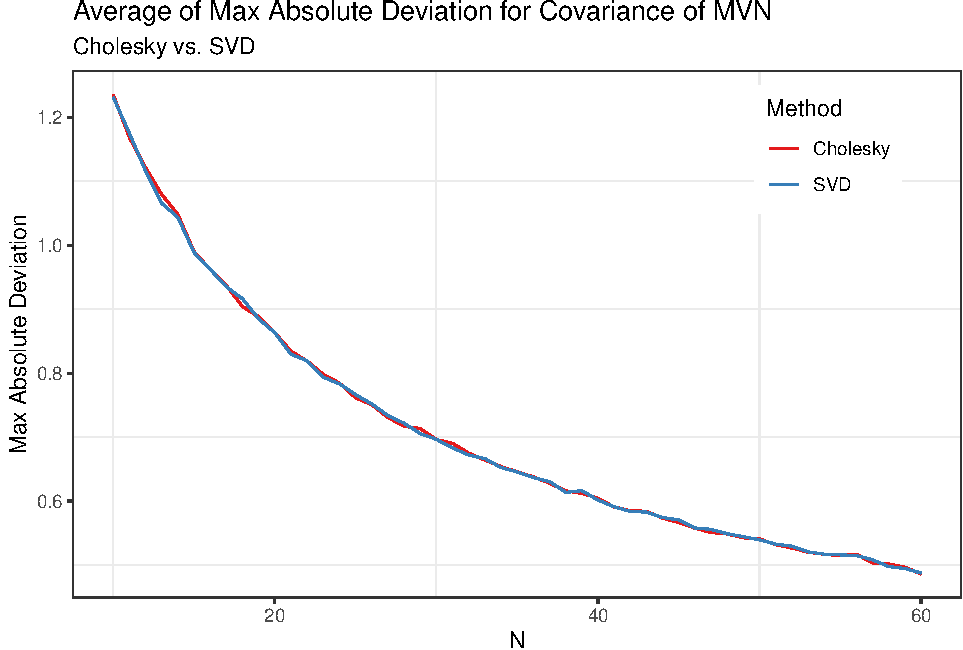
\includegraphics{mvnorm_files/figure-latex/unnamed-chunk-7-1.pdf}

Lastly, then, the two approaches are equal on average, even in small
samples.

\hypertarget{endnotes}{%
\section{Endnotes}\label{endnotes}}

\end{document}
